\documentclass[tikz,border=3mm]{standalone}
\usepackage[utf8]{inputenc}
\usepackage[T1]{fontenc}
\usepackage{helvet}
\renewcommand{\familydefault}{\sfdefault}
\usetikzlibrary{arrows.meta,positioning}
\begin{document}

\tikzset{every node/.append style={font=\sffamily\small}}
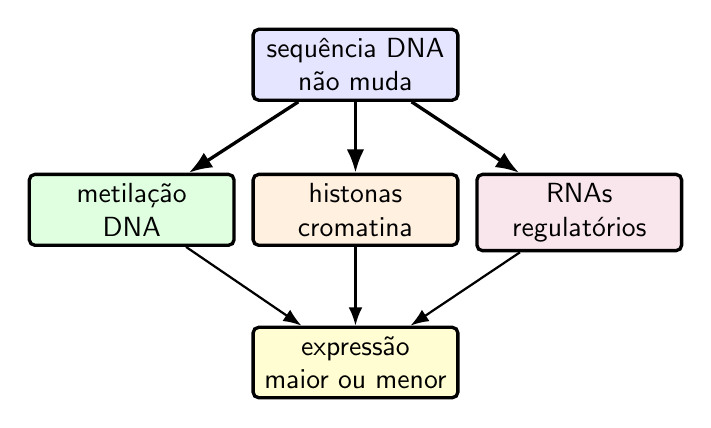
\begin{tikzpicture}[>=Latex,node distance=0.75cm]
  \tikzstyle{box}=[draw,rounded corners=2pt,very thick,align=center,minimum width=2.6cm,minimum height=0.75cm]
  \node[box,fill=blue!10] (seq) {sequência DNA\\não muda};
  \node[box,fill=green!12,below left=0.9cm and 0.2cm of seq] (met) {metilação\\DNA};
  \node[box,fill=orange!12,below=0.9cm of seq] (his) {histonas\\cromatina};
  \node[box,fill=purple!10,below right=0.9cm and 0.2cm of seq] (rna) {RNAs\\regulatórios};
  \node[box,fill=yellow!18,below=1.0cm of his] (exp) {expressão\\maior ou menor};
  \draw[very thick,->] (seq) -- (met);
  \draw[very thick,->] (seq) -- (his);
  \draw[very thick,->] (seq) -- (rna);
  \draw[thick,->] (met) -- (exp);
  \draw[thick,->] (his) -- (exp);
  \draw[thick,->] (rna) -- (exp);
\end{tikzpicture}
\end{document}
